% File: disjoint-paths-step-ladder.tex
\documentclass{standalone}

\usepackage{amssymb}
\usepackage{tikz}
\usetikzlibrary{shapes, positioning, arrows.meta, calc, backgrounds, fit, decorations.pathmorphing}

% default horizontal/vertical distance
\def\hdist{1.0}
\def\vdist{1.0}

\def\hdistval{0.8}
\def\vdistval{1.0}

\def\hladderdistval{0.20}

\newcommand{\state}[3]{% #1: state name; #2: position; #3: state label
  \node (#1) [circle, inner sep = 0pt, minimum size = 8mm, text width = 8mm, align = center, draw, #2, font = \Large] {#3};
}

\newcommand{\handrail}[2]{ %1: new-state/pre; % direction
  \foreach \name/\pre/\label in {#1} {
    \state{\name}{below #2 = \vdistval*\vdist and \hdistval*\hdist of \pre}{\label}
	\draw[>=Stealth, ->] (\pre) to (\name);
  }
}

\newcommand{\cross}[1]{
  \foreach \unprime in {#1} {
	\draw[>=Stealth, ->] (\unprime') to node [above, font = \large] {$o$} (\unprime);
  }
}

\newcommand{\join}[2]{
  \draw[>=Stealth, ->] (#1) edge (#2) (#1') edge (#2');
}

% #1: color (for example)
\tikzset{path/.style = {>=Stealth, ->, very thick, #1, decorate, decoration = {snake, post length = 1mm}}}
\tikzset{edge/.style = {>=Stealth, ->, very thick, #1}}
\tikzset{op/.style = {font = \Large}}

\begin{document}
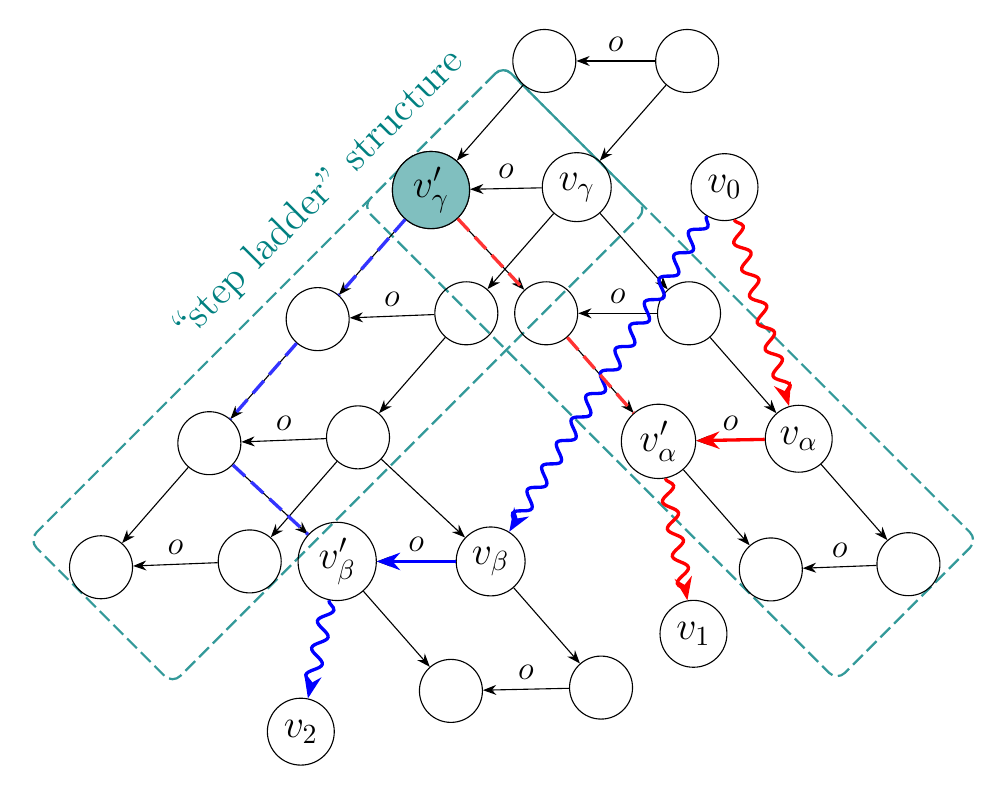
\begin{tikzpicture}
  \begin{scope}	% draw the ladders
    % the ladder on the left
    \state{s0}{}{}
    \state{s0'}{right = of s0}{}
    % first 4: left handrail; last 4: right handrail
	\handrail{s1/s0/$v'_{\gamma}$, s2/s1/, s3/s2/, s4/s3/, s1'/s0'/$v_{\gamma}$, s2'/s1'/, s3'/s2'/, s4'/s3'/}{left}
    % cross steps
    \cross{s0, s1, s2, s3, s4}

    % the ladder on the right
    \state{s5}{right = \hladderdistval*\hdist of s2'}{}
    \state{s5'}{right = of s5}{}
    % first 2: left handrail; last 2: right handrail
	\handrail{s6/s5/$v'_{\alpha}$, s7/s6/, s6'/s5'/$v_{\alpha}$, s7'/s6'/}{right}
    % cross steps
    \cross{s5, s6, s7}

    % the ladder at the bottom
	\state{s8}{right = \hladderdistval*\hdist of s4'}{$v'_{\beta}$}
	\state{s8'}{right = of s8}{$v_{\beta}$}
    % first 1: left handrail; last 1: right handrail
    \handrail{s9/s8/, s9'/s8'/}{right}
    % cross steps
    \cross{s8, s9}

    % join the left and the right ladders
    \join{s1}{s5}
    \join{s3}{s8}
  \end{scope}

  \begin{scope} % sig0 = LCA(sig1, sig2)
	\state{sig0}{right = of s1'}{$v_0$}

	\state{sig1}{below right = 1.8*\vdist and -0.2*\hdist of s6}{$v_{1}$}
	\draw (sig0) edge[path = {red}] (s6') 
		(s6') edge[edge = {red}] (s6) 
		(s6) edge[path = {red}] (sig1);

	\state{sig2}{below left = 1.5*\vdist and -0.2*\hdist of s8}{$v_{2}$}
	\draw (sig0) edge[path = {blue}] (s8') 
		(s8') edge[edge = {blue}] (s8) 
		(s8) edge[path = {blue}] (sig2);
  \end{scope}

  % siggamma = LCA(sig1, sig2)
  \begin{scope}[conn/.style = {#1, very thick, dash pattern = on 6pt off 3pt}] 
	\state{siggamma}{at = (s1), fill = teal!50, inner sep = 0pt}{$v'_{\gamma}$}
	\draw[conn = {blue!80}] (siggamma) edge (s2) 
		(s2) edge (s3)
		(s3) edge (s8);
	\draw[conn = {red!80}] (siggamma) edge (s5) 
		(s5) edge (s6);
  \end{scope}

  % step ladder structure
  \begin{scope}[bg/.style = {rectangle, rounded corners, dash pattern = on 5pt off 2pt, thick, draw = teal!80}]
	\begin{pgfonlayer}{background}
	  \node (left) [bg, rotate fit = 45, fit = (s1) (s1') (s4) (s4'), 
		label = {[rotate = 45, font = \Large, teal, above = 5pt] 45:``step ladder'' structure}] {};
	  \node (right) [bg, rotate fit = 45, fit = (s1) (s1') (s7) (s7')] {};
	\end{pgfonlayer}
  \end{scope}
\end{tikzpicture}
\end{document}
